\begin{knitrout}
\definecolor{shadecolor}{rgb}{0.969, 0.969, 0.969}\color{fgcolor}\begin{figure}

{\centering 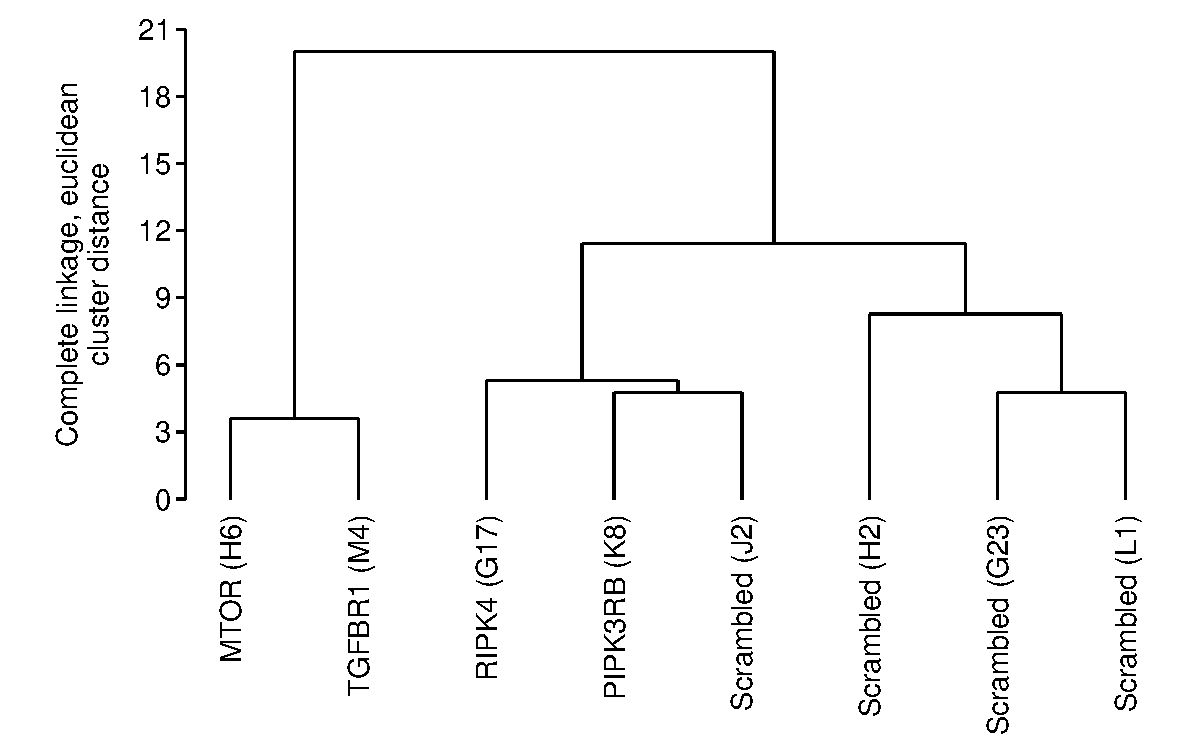
\includegraphics[width=.7\linewidth]{figures/R/forest-tree-forest-tree-1} 

}

\caption[Hierarchical clustering on averaged random forest importance scores of cellular features.]{Complete linkage hierarchical clustering performed on euclidean distances from cell feature importance scores, obtained through random forest analysis and averaged by well. For each gene and scrambled well, all available 8 replicates of the \textit{Brucella} Dharmacon unpooled dataset were considered.}\label{fig:forest-tree}
\end{figure}


\end{knitrout}

